\section{HybridGuard}
\label{sec:method}
\begin{figure*}[t]
\centering
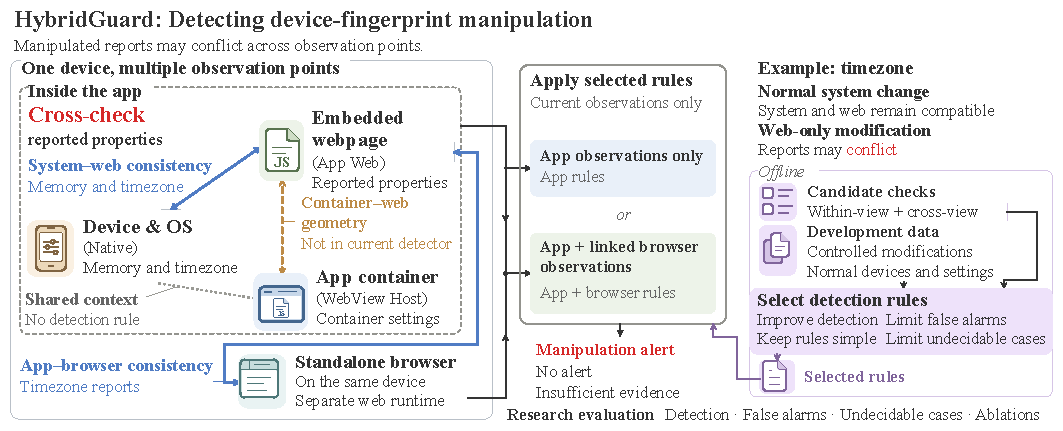
\includegraphics[width=\textwidth]{figures/overview.pdf}
\caption{HybridGuard uses complementary observations from the same device to check fingerprint reports. Offline selection constrains normal alarms and definite-output coverage; frozen detectors consume current App observations or linked App--browser observations. Solid comparison edges denote detector relations. Host--Web geometry is a separate study; the dotted Native--Host edge supplies context only. No surface is trusted ground truth. No alert does not establish safety, and execution failures are recorded separately.}
\Description{Android Native, WebView host, and App Web observations form a triangle. An external browser joins through a pairing step. Offline constrained selection supplies detectors, whose outputs are alert, no alert, or insufficient evidence. A timezone example contrasts a normal system change with a webpage-only modification.}
\label{fig:overview}
\end{figure*}

\subsection{Collection and State-Aware Checks}
Figure~\ref{fig:overview} separates measurement, offline selection, and current-record evaluation. Each field carries a value and an observation status. Normalization handles units and schema versions before a check executes; unsupported, missing, or unparsable operands remain unavailable. Original records, receipts, and pairing metadata support source attribution. A paired view requires two linked observations; an incomplete browser capture leaves an App-only record rather than a fabricated browser vector. Pair identifiers, experiment labels, environment names, and stage metadata are excluded from prediction inputs.

A check is a predicate together with its prerequisites and interpretation. Candidate conditions include single-field thresholds, relations within the App Web view, and Native--Web references. A reference is not an instruction to require exact equality: measurements may be bucketed, unit-converted, or tied to a collection interval. Documentation informs these interpretations, while project predicates and tolerances remain research choices rather than official attack rules.

Let $r_j(x)\in\{\hgstate{T},\hgstate{F},\hgstate{U},\hgstate{FAILED}\}$ be the state of a selected condition on current observation $x$. The detector is an OR of selected singleton conditions. After checking selected-input validity, any execution or binding failure yields \hgstate{FAILED}; otherwise any \hgstate{T} yields an alert, all \hgstate{F} yields no alert, and the remaining cases yield \hgstate{U}. An empty selected set has its own status. Thus a known violation can establish an alert despite another unknown condition, whereas unknown evidence cannot establish a definite no-alert result. Unselected fields do not independently cause failure.

\subsection{Device References}
\paragraph{Memory.}
The memory reference tests whether a positive Web-reported memory value exceeds a coarse upper envelope of observed Native memory:
\begin{equation}
 r_{\mathrm{mem}}(x) = \big[m_{\mathrm{web}}>2^{\lceil\log_2 m_{\mathrm{native}}\rceil}\big].
\label{eq:memory}
\end{equation}
Both operands are expressed in GiB, and validity checks include a Native value of at least 0.25 GiB. The envelope accommodates coarse reporting instead of demanding physical-memory equality. It targets upward violations; a smaller or coordinated plausible report can evade it. We compare it with the fixed condition $m_{\mathrm{web}}>8$ in a separate mechanism study.

\paragraph{Timezone.}
The Native timezone reference derives the effective offset from the device's IANA timezone and its collection interval, using the fixed timezone database 2026c. It compares this offset with the Web \texttt{getTimezoneOffset} value after reversing the UTC-offset sign convention. It compares effective offsets, not timezone-name strings. An ambiguous transition interval or unusable prerequisite yields unknown; zero and minus one are not automatically missing sentinels. This permits an ordinary system timezone change when both observations move consistently, while exposing a Web-only override that does not match the Native reference.

\paragraph{Host geometry.}
A separate check compares visual-viewport geometry with a host measurement of the containing View. For either axis, let $P$ be the CSS visual-viewport size multiplied by device-pixel ratio and visual-viewport scale, and let $H$ be the host View size less its own padding. The check alerts if $P>H+\epsilon$, with $\epsilon=2+4\cdot2^{-23}\max(|P|,|H|,1)$ pixels. Snapshot binding and host-before/after stability are prerequisites. The implemented domain also requires an attached, visible host View, zero padding, and an identity View transform; observations outside that domain yield unknown. This fixed engineering tolerance is not a platform guarantee. The condition is evaluated as a specialist mechanism and is \emph{not} part of \full.

\subsection{Constrained Detector Selection}
The App pool contains 50 base templates and three fixed relations, expanded using the training-side encoder and admissible polarities. The full pool has 65, 65, and 56 expanded atoms across the three model configurations. A candidate must be sufficiently assessable on historical normal training data; absence of a comparable field is not resolved by assuming that the condition is false.

For a selected set $S$, the sparse stage maximizes the heuristic objective
\begin{equation}
 J(S)=\frac{1}{K}\sum_{k=1}^{K}\overline{d}_k(S)-0.005\,C(S),
\label{eq:selection}
\end{equation}
where $K=14$, $\overline{d}_k$ averages detection over training environments and then effective modification positions within configuration $k$, and $C$ counts clauses plus literal occurrences. Selection uses greedy improving additions, retains the best feasible prefix, and performs a backward-pruning pass; it does not guarantee a global optimum.

Feasibility limits a detector to eight singleton OR clauses, complexity 16, and two clauses per registered family, without opposite polarities of the same atom. Separate training-normal alarm budgets are $\lfloor0.05\cdot168\rfloor=8$ for controlled records and $\lfloor0.05\cdot630\rfloor=31$ for historical cloud-device records. Candidate assessability and final definite-output coverage on the latter must each reach 90\%; controlled coverage is constrained per phase at 80\%. Fitting disallows execution failures and uses a 60-second deadline per fit.

The subsequent retention stage starts from that configuration's sparse solution. It can add semantic diversity without losing training detections, or replace a same-group condition with a registered higher-quality alternative under per-record nonregression checks. It does not continue optimizing Equation~\ref{eq:selection}. We evaluate the saved retention outputs consistently, rather than choosing a stage separately for each result cell. The resulting detector is frozen before its designated evaluations.

\subsection{Paired Browser Extension}
The retained paired detector adds a cross-endpoint timezone condition, C1, to the frozen App detector. C1 alerts when the linked App Web and external-browser offsets are unequal. Both are finite numeric Web offsets with the same sign convention; zero and minus one are valid. C1 has no timestamp gate, unlike the interval-aware Native timezone reference. Missing or inapplicable evidence remains unknown under the same state-aware combination. The extension selection compared the empty set, C1, a language condition C2, and their combination, with separate normal-alarm budgets of 31/630 MTC training records, 0/12 pilot normals, and 1/34 matched normals, plus 90\% definite-output coverage. C2 alarms on two matched normal preference changes, and the two-condition combination provides only 566/630 definite MTC training outputs; neither meets the frozen constraints. This offers a second endpoint for testing a mismatch; it does not establish which endpoint is truthful or make language differences suspicious by definition. The extension is evaluated separately from the App benchmark because the original App positions do not have contemporaneous external-browser counterparts.
